%	$Id$	
%%%%%%%%%%%%%%%%%%%%%%%%%%%%%%%%%%%%%%%%%%%%%%%%%%%%%%%%%%%%%%%%%%%
%                                                                 %
%   HBOOK User Guide -- LaTeX Source                              %
%                                                                 %
%   Chapter 1                                                     %
%                                                                 %
%   The following external EPS files are referenced:              %
%         hbbatch.eps, hbookc11.eps                               %
%                                                                 %
%   Editor: Michel Goossens / CN-AS                               %
%   Last Mod.: 20 October 1993  9:00 mg                           %
%                                                                 %
%%%%%%%%%%%%%%%%%%%%%%%%%%%%%%%%%%%%%%%%%%%%%%%%%%%%%%%%%%%%%%%%%%%

\chapter{Introduction}       
\label{HINTRO}
 
Data processing is an important aspect of particle physics experiments
since the volume of data to be handled is quite large, a single LEP 
experiment producing of the order of a terabyte of data per year.
As a result, every particle physics laboratory has a large data 
processing centre even though more than 50\% of the computation is
actually carried on in universities or other research establishments.  
Particle physicists from various countries are in close contact on 
a continental and world wide basis,
the information exchanged being mainly via preprints and conferences.
The similarities in experimental devices and problems, and the close
collaboration, favour the adoption of common software methodologies that
sometimes develop into widely used standard packages. 
Examples are the histograming, fitting and data presentation package HBOOK, its
graphic interface \HPLOT~\cite{bib-HIGZHPLOT} and the
Physics Analysis Workstation (\PAW) system~\cite{bib-PAW}, 
which have been developed at CERN.

HBOOK is a subroutine package to handle statistical distributions
(histograms and Ntuples) in a Fortran scientific computation environment. 
It presents results graphically on the line printer, and can
optionally draw them on graphic output devices via the \HPLOT{}
package.
\PAW{} integrates the functionalities of the \HBOOK{} 
and \HPLOT{} (and other) packages
into an interactive workstation environment and provides the 
user with a coherent and complete working environment, 
from reading a (mini)DST,
via data analysis to preparing the final data presentation.

These packages are available from the CERN Program Library 
(see the copyright page for conditions).
They are presently being used on several hundred different computer
installations throughout the world.

\section{Data processing flow in particle experiments}
\label{HDATPROC}

In the late sixties and early seventies a large fraction of particle 
physicists were active in bubble chamber physics.
The number of events they treated varied between a few hundreds (neutrino) 
to several tens of thousands (e.g. strong interaction spectroscopy). 
Normally users would reduce there raw ``measurement'' tapes
\index{DST}
after event reconstruction onto Data Summary Tapes (DST) and extract from
there mini and micro DSTs, which would then be used for analysis.
In those days a statistical analysis program SUMX~\cite{bib-SUMX}
would read each event and compile information into histograms,
two-dimensional scatter diagrams and `ordered lists'. Facilities were
provided (via data cards) to select subset of events according
to criteria and the user could add routines for computing, event by
event, quantities not immediately available.

Although the idea and formalism of specifying cuts and
selection criteria in a formal way were a very nice idea,
the computer technology of those days only allowed the data to be analysed
in batch mode on the CDC or IBM mainframes.
Therefore it was not always very practical to run several times
through the data and a more lightweight system 
HBOOK~\cite{bib-HBOOK1,bib-HBOOK2},
easier to learn and use, was soon developed.

It was in the middle seventies, when larger proton and electron
accelerators became available, that counter experiments 
definitively superseded bubble chambers and with them the amount of data
to be treated was now in the multi megabyte range. Thousands of
raw data tapes would be written, huge reconstruction programs would
extract interesting data from those tapes and transfer them to 
DSTs. Then, to make the analysis more manageable, various physicists
would write their own mini-DST, with a reduced fraction of the
information from the DST. They would run these (m,$\mu$)DSTs through
HBOOK, whose functionality had increased substantially
in the meantime~\cite{bib-HBOOK3,bib-HBOOK3R}.
Hence various tens of one- or two-dimensional histograms
would be booked in the initialization phase and the interesting
parameters would be read sequentially from the DST and
be binned in the histograms or scatter plots. 
Doing this was very efficient memory wise (although 2-dim.
histograms could still be very costly), but of course all correlations,
not explicitly plotted, were lost.

HBOOK in those days still had its own memory management, but with 
version~4~\cite{bib-HBOOK4}, which became available in 1984, the
ZEBRA data memory manager was introduced.
This not only allowed the use of all memory managament facilities of ZEBRA,
but at the same time it became possible to use the sequential 
FZ and random access RZ~\cite{bib-ZEBRA} input-output
possiblities of that system.
This allows ``histograms'' to be saved and transferred to other systems
in an easy way.
At about the same time Ntuples, somewhat similar in functionality to 
``events'' as written on a miniDST were implemented.
This way the complete correlation matrix between the various
Ntuple elements can be reconstructed at will. 
The last few years multi Mflop machines have become available
on the desktop, and ``farms'' of analysis machines are being set up
to ``interactively'' reconstruct events directly from the
raw data as registered in the experimental setup, hence bypassing the
``batch'' reconstruction step.
The first Ntuple implementation can be thought of as a static large
two-dimensional array, one dimension representing the number of events
and the other a number of characteristics (floating point numbers)
stored for each event. 
With the present version of HBOOK Ntuples can contain complex
substructures of different data types, which allow a certain dynamicity.
Moreover tools have been developed to dynamically share
data between various processes (Unix) or global sections (VMS).
This makes it now possible to sample events as they are registered 
in the experimental setup or, when the computing power is
available, to reconstruct, vizualise and analize events in real time
as they are recorded in the experimental apparatus.
It is expected that this will progressively eliminate the intermediate
Batch/DST analysis step and allow, with the help of Monte Carlo events 
and calibration data, an (almost) immediate response to the
data taking needs of a large experiment.

\section{HBOOK and its output options}
\label{HOUTOPTS}

The HBOOK system consists of a few hundred Fortran
subroutines which enable the user to symbolically define, fill and output
one- and two-dimensional density estimators, under the form
of {\bf histograms}, {\bf scatter-plots} and {\bf tables} and
to handle Ntuples.

\index{histogram}
\index{scatter-plot}
\index{table}
\index{Ntuple}

Some interesting features of HBOOK are:
\begin{UL}
\item The basic operations require the knowledge of just a few
      subroutine calls that can be learned in half an hour, reading a few
      pages of documentation.  
      The internal structure of the
      package is also such that the options that are not directly
      called by the user program are not loaded in memory.
\item Histograms and plots are represented on the line printer in a
      standard format that contains the picture and some numerical 
      information. 
      Several options are available to modify the presentation, 
      mainly in the case of one dimensional histograms.  
      By default, one histogram per page is printed,
      writing a possible common title, date, individual title, drawing
      the countour of the histogram between the minimum and maximum
      channel content, with the contents scale adjusted to fit in one
      page, followed by channel number, contents and scale, and some
      statistical information (entries, mean value, standard deviation
      and so on).  
      If the number of channels is greater than 100, the
      histogram is printed on several pages.
\item Printing options permit to add or suppress some information,
      choose a different graphic presentation and modify the mapping of
      histograms on output pages.  
      Histograms can also be printed with channels
      oriented along rows instead of columns, to avoid splitting the
      ones with many channels. 
      Logarithmic contents scale can be selected.
      Various alternative output choices are illustrated in the examples.
\end{UL}

About 120 subroutines are directly accessible to the user program, via
Fortran calls of the type

\begin{center}
\fbox{\Lit{CALL H.....(P1,P2,..)}}
\end{center}

This is the only interface between a Fortran program and the dynamic
data structure managed by HBOOK, which thus
remains hidden from the average user.

\subsection*{The functionality of HBOOK}
      
The various user routines of HBOOK can be subdivided by functionality
as follows:
\begin{DL}{Random number generation}
\item[Booking]
      Declare a one- or two-dimensional histogram or a Ntuple.
\item[Projections]
      Project two-dimensional distributions onto both axes.
\item[Ntuples]
      Way of writing micro data-summary-files for further
      processing. This allows projections of
      individual variables or correlation plots. Selection mechanisms
      may be defined.
\item[Function representation]
      Associates a real function of 1 or 2 variables to a histogram.
\item[Filling]
      Enter a data value into a given histogram, table or Ntuple.
\item[Access to information]
      Transfer of numerical values from HBOOK-managed memory to Fortran
      variables and back.
\item[Arithmetic operations]
      On histograms and Ntuples.
\item[Fitting]
      Least squares and maximum likelihood fits of
      parametric functions to histogramed data.
\item[Monte Carlo testing]
      Fitting with finite Monte Carlo statistics.
\item[Differences between histograms\quad]
      Statistical tests on the compatibility in shape between histograms
      using the Kolmogorov test.
\item[Parameterization]
      Expresses relationships between as linear combinations of elementary
      functions. 
\item[Smoothing]
      Splines or other algorithms.
\item[Random number generation]
      Based on experimental distributions.
\item[Archiving]
      Information is stored
      on mass storage for further reference in subsequent programs.
\item[Editing]
      Choice of the form of presentation of the histogramed data.
\end{DL}

\section{What you should know before you start}

The basic data elements of HBOOK are the {\bf histogram} (one-
and two-dimensional) and the {\bf Ntuple}. The user identifies
his data elements using a {\bf single integer}. Each of the
elements has a number of {\bf attributes} associated with it.
\index{histogram}
\index{Ntuple}

The package is organised as part of a {\bf library}, from which
at load time unsatisfied externals are searched and loaded.
In this way only those subroutines actually used will be
loaded, therefore minimising the space occupied in memory by the code.
Unfortunately, given the way Fortran
works and although the package is structured as much as possible in the
sense of selective loading, some unused subroutines will usually be
present.

\finalnewpage

HBOOK uses the ZEBRA \cite{bib-ZEBRA} data structure
management package to manage its memory (see chapter \ref{HMEMORYM}).
The working space of HBOOK is an array, allocated to the labelled
common \Lit{/PAWC/}.
\index{common {\tt/PAWC/}}\index{PAWC@{\tt/PAWC/} common}
In ZEBRA terms this is a ZEBRA store.
It is thus necessary to reserve as many locations as required with a
declarative statement in the main program.
The actual length of the common is defined most safely via 
a \Lit{PARAMETER} statement, as shown below:

\begin{center}
\begin{tabular}{|>{\tt}l|}
\hline
PARAMETER (NWPAWC = 50000)\\
COMMON /PAWC/ HMEMOR(NWPAWC)\\
\hline
\end{tabular}
\end{center}
\index{common {\tt/PAWC/}}\index{PAWC@{\tt/PAWC/} common}

Furthermore HBOOK must be informed of the storage 
limit via a call to \Rind{HLIMIT}.
This is discussed in detail in section \vref{HMEMORYS}.
In the case above this would correspond to

\begin{center}
\fbox{CALL HLIMIT(NWPAWC)}
\end{center}
\Rind[HLIMIT]{}
 
At execution time, when histograms are booked, they are accomodated
in common \Lit{/PAWC/} in booking order, up to the maximum size available.
\index{common {\tt/PAWC/}}\index{PAWC@{\tt/PAWC/} common}

Note that a call to \Rind{HLIMIT} will automatically initialise the ZEBRA system
via a call to the routine \Rind{MZEBRA}.
If ZEBRA has already been initialised, (\Rind{MZEBRA} has already been called),
then \Rind{HLIMIT} should be called with a
{\bf negative} number indicating the number of words required, e.g.

\begin{center}
\fbox{CALL HLIMIT(-NWPAWC)}
\end{center}
\Rind[HLIMIT]{}

\subsection{HBOOK parameter conventions}

\subsubsection*{Histogram or Ntuple Identiers}
 
Histograms and Ntuples in HBOOK are identified by a positive 
or negative integer.
Thus the histogram identifier \Lit{ID = 0} is illegal at {\bf booking} time.
However it is a convenient way to specify that the option or operation
applies to {\bf all} known histograms in the current
working directory (e.g. output, input, printing).
All routines for which a zero identifier is meaningful
are mentioned explicitly.
\index{histogram!identifier}
\index{Ntuple!identifier}
\index{identifier}

\subsubsection*{Parameter types}

In agreement with the Fortran standard, when calling an
HBOOK routine the type of each parameter must correspond to
the one described in the routine's calling sequence in this manual.
Unless explicitly stated otherwise, parameters whose  names
start with \Lit{I, J, K, L, M} or \Lit{N} are {\bf integer}, 
the rest {\bf real}, with the exception of those beginning 
with the string \Lit{CH}, which correspond to character constants. 
\index{parameter type}
\index{Fortran convention}
\index{real type}
\index{character  type}
\index{integer type}
\index{type!parameter}
\index{type!real}
\index{type!character type}
\index{type!integer}

\subsubsection*{Data packing}
\index{packing}
\index{VMX@{\tt VMX}}

All booking commands that reserve space for histograms or plots
require the ``packing'' parameter \Lit{VMX}.
It corresponds to the 
estimated maximum population of a single bin,
on the basis of which a suitable number of bits per channel will be
allocated.
This allows several channels to be packed in one machine word,
and thus to require less storage space (at the expense of packing
and unpacking processing time).
A value \Lit{VMX=0.0} signals that no packing is to be performed
and that each histogram channel will occupy one machine word.

\finalnewpage

\section{A basic example}
\label{HSIMPLEXA}

Below a simple example is given describing 
how to use HBOOK for booking, filling and printing simple histograms.
After telling HBOOK the length of the \Lit{/PAWC/} common block
\index{common {\tt/PAWC/}}\index{PAWC@{\tt/PAWC/} common}
to be \Lit{10000} words with a call to \Rind{HLIMIT}, a 
global title to appear on all histograms is specified by calling
\Rind{HTITLE}. 
Next a 100 bin one-dimensional histogram with identifier 10 is booked 
with a call to \Rind{HBOOK1}, followed by the booking 
using a call to \Rind{HBOOK2} of a two-dimensional histogram with identifier 20 
and consisting of 100 times 40 cells.
The \Lit{DO}-loop labelled 10 fills the one-dimensional histogram 10,
while the nested \Lit{DO} loops labelled 20 and 30 look after filling
the two-dimensional histogram 20. 
In both cases a call is made to routine \Rind{HFILL}.
Finally a call to \Rind{HISTDO} writes an index with information 
about all histograms as well as a lineprinter representation of
the histograms on standard output.

\begin{XMPt}{Example of how to produce simple histograms}
      PROGRAM HSIMPLE
*
      PARAMETER (NWPAWC = 10000)
      COMMON/PAWC/H(NWPAWC)
*.___________________________________________
      CALL HLIMIT(NWPAWC)
*                       Set global title
*
      CALL HTITLE('EXAMPLE NO = 1')
*                       Book 1-dim histogram and scatter-plot
*
      CALL HBOOK1(10,'EXAMPLE OF 1-DIM HISTOGRAM',100,1.,101.,0.)
      CALL HBOOK2(20,'EXAMPLE OF SCATTER-PLOT',100,0.,1.,40,1.,41.,30.)
*                       Fill 1-dim histogram
*
      DO 10 I=1,100
         W=10*MOD(I,25)
         CALL HFILL(10,FLOAT(I)+0.5,0.,W)
  10  CONTINUE
*                       Fill scatter-plot
*
      X=-0.005
      DO 30 I=1,100
         X=X+0.01
         DO 20 J=1,40
            Y=J
            IW=MOD(I,25)*MOD(J,10)
            IWMAX=J-MOD(I,25)+10
            IF(IW.GT.IWMAX)IW=0
            CALL HFILL(20,X,Y,FLOAT(IW))
  20     CONTINUE
  30  CONTINUE
*                       Print all histograms with an index
*
      CALL HISTDO
      END
\end{XMPt}
\finalnewpage%%%%%%%%%%%%%%%%%%%%%%%%%%%%%%%%%%%%%%%%%%%%%%%%%%%%%%%%%%%%%%%%%%%%%%%%%%%%%%%%%%%%%%
\begin{Listing}
 EXAMPLE NO = 1
 
 .............................................................................................................................
 .                                                                                                                           .
 .   HBOOK   HBOOK  CERN            VERSION   4.13       HISTOGRAM AND PLOT INDEX                             17/12/91       .
 .                                                                                                                           .
 .............................................................................................................................
 .                                                                                                                           .
 .  NO                     TITLE                      ID  B/C  ENTRIES DIM   NCHA     LOWER       UPPER       ADDRESS LENGTH .
 .                                                                                                                           .
 .............................................................................................................................
 .                                                                                                                           .
 .                                                                                                                           .
 .   1  EXAMPLE OF 1-DIM HISTOGRAM                    10  32      100  1  X   100   0.100E+01   0.101E+03       79369    149 .
 .                                                                                                                           .
 .                                                                                                                           .
 .   2  EXAMPLE OF SCATTER-PLOT                       20   5     4000  2  X   100   0.000E+00   0.100E+01       79217    760 .
 .                                                                        Y    40   0.100E+01   0.410E+02       78482    726 .
 .                                                                                                                           .
 .............................................................................................................................

 MEMORY UTILISATION

      MAXIMUM TOTAL SIZE OF COMMON /PAWC/            80000
\newpage\setlength{\baselineskip}{5.7pt}\relax
 EXAMPLE NO = 1                                                                  
 --------------                                                                  
 EXAMPLE OF 1-DIM HISTOGRAM                                                      
 
 HBOOK     ID =        10                                        DATE  17/12/91              NO =   1
 
      250
      240                              -                        -                        -                        -
      230                             -I                       -I                       -I                       -I
      220                            -II                      -II                      -II                      -II
      210                           -I I                     -I I                     -I I                     -I I
      200                          -I  I                    -I  I                    -I  I                    -I  I
      190                         -I   I                   -I   I                   -I   I                   -I   I
      180                        -I    I                  -I    I                  -I    I                  -I    I
      170                       -I     I                 -I     I                 -I     I                 -I     I
      160                      -I      I                -I      I                -I      I                -I      I
      150                     -I       I               -I       I               -I       I               -I       I
      140                    -I        I              -I        I              -I        I              -I        I
      130                   -I         I             -I         I             -I         I             -I         I
      120                  -I          I            -I          I            -I          I            -I          I
      110                 -I           I           -I           I           -I           I           -I           I
      100                -I            I          -I            I          -I            I          -I            I
       90               -I             I         -I             I         -I             I         -I             I
       80              -I              I        -I              I        -I              I        -I              I
       70             -I               I       -I               I       -I               I       -I               I
       60            -I                I      -I                I      -I                I      -I                I
       50           -I                 I     -I                 I     -I                 I     -I                 I
       40          -I                  I    -I                  I    -I                  I    -I                  I
       30         -I                   I   -I                   I   -I                   I   -I                   I
       20        -I                    I  -I                    I  -I                    I  -I                    I
       10       -I                     I -I                     I -I                     I -I                     I
 
 CHANNELS 100   0                                                                                                  1   
           10   0        1         2         3         4         5         6         7         8         9         0   
            1   1234567890123456789012345678901234567890123456789012345678901234567890123456789012345678901234567890   
 
 CONTENTS 100            111111111122222          111111111122222          111111111122222          111111111122222 
           10   123456789012345678901234 123456789012345678901234 123456789012345678901234 123456789012345678901234 
            1.  000000000000000000000000 000000000000000000000000 000000000000000000000000 000000000000000000000000 
 
 LOW-EDGE 100                                                                                                      1
           10            1111111111222222222233333333334444444444555555555566666666667777777777888888888899999999990
            1.  1234567890123456789012345678901234567890123456789012345678901234567890123456789012345678901234567890
 
 * ENTRIES =        100      * ALL CHANNELS = 0.1200E+05      * UNDERFLOW = 0.0000E+00      * OVERFLOW = 0.0000E+00
 * BIN WID = 0.1000E+01      * MEAN VALUE   = 0.5433E+02      * R . M . S = 0.2854E+02

\finalnewpage

 EXAMPLE NO = 1                                                                  
 --------------                                                                  
 
 EXAMPLE OF SCATTER-PLOT                                                         
 
 HBOOK     ID =        20                                        DATE  17/12/91              NO =   2
 
 CHANNELS 100 U 0                                                                                                  1 O 
           10 N 0        1         2         3         4         5         6         7         8         9         0 V 
            1 D 1234567890123456789012345678901234567890123456789012345678901234567890123456789012345678901234567890 E 
            ************************************************************************************************************
   OVE      *                                                                                                          * OVE
    40      *                                                                                                          *  40
    39      *   9IR*                     9IR*                     9IR*                     9IR*                        *  39
    38      *   8GO**                    8GO**                    8GO**                    8GO**                       *  38
    37      *   7ELS*                    7ELS*                    7ELS*                    7ELS*                       *  37
    36      *   6CIOU*                   6CIOU*                   6CIOU*                   6CIOU*                      *  36
    35      *   5AFKPU*                  5AFKPU*                  5AFKPU*                  5AFKPU*                     *  35
    34      *   48CGKOS*                 48CGKOS*                 48CGKOS*                 48CGKOS*                    *  34
    33      *   369CFILORU               369CFILORU               369CFILORU               369CFILORU                  *  33
    32      *   2468ACEGIKMOQS           2468ACEGIKMOQS           2468ACEGIKMOQS           2468ACEGIKMOQS              *  32
    31      *   +23456789ABCDEFGHIJK     +23456789ABCDEFGHIJK     +23456789ABCDEFGHIJK     +23456789ABCDEFGHIJK        *  31
    30      *                                                                                                          *  30
    29      *   9IR                      9IR                      9IR                      9IR                         *  29
    28      *   8GO*                     8GO*                     8GO*                     8GO*                        *  28
    27      *   7ELS                     7ELS                     7ELS                     7ELS                        *  27
    26      *   6CIOU                    6CIOU                    6CIOU                    6CIOU                       *  26
    25      *   5AFKP                    5AFKP                    5AFKP                    5AFKP                       *  25
    24      *   48CGKO                   48CGKO                   48CGKO                   48CGKO                      *  24
    23      *   369CFILO                 369CFILO                 369CFILO                 369CFILO                    *  23
    22      *   2468ACEGIK               2468ACEGIK               2468ACEGIK               2468ACEGIK                  *  22
    21      *   +23456789ABCDEF          +23456789ABCDEF          +23456789ABCDEF          +23456789ABCDEF             *  21
    20      *                                                                                                          *  20
    19      *   9I                       9I                       9I                       9I                          *  19
    18      *   8GO                      8GO                      8GO                      8GO                         *  18
    17      *   7EL                      7EL                      7EL                      7EL                         *  17
    16      *   6CI                      6CI                      6CI                      6CI                         *  16
    15      *   5AFK                     5AFK                     5AFK                     5AFK                        *  15
    14      *   48CG                     48CG                     48CG                     48CG                        *  14
    13      *   369CF                    369CF                    369CF                    369CF                       *  13
    12      *   2468ACE                  2468ACE                  2468ACE                  2468ACE                     *  12
    11      *   +23456789A               +23456789A               +23456789A               +23456789A                  *  11
    10      *                                                                                                          *  10
     9      *   9                        9                        9                        9                           *   9
     8      *   8G                       8G                       8G                       8G                          *   8
     7      *   7E                       7E                       7E                       7E                          *   7
     6      *   6C                       6C                       6C                       6C                          *   6
     5      *   5A                       5A                       5A                       5A                          *   5
     4      *   48                       48                       48                       48                          *   4
     3      *   369                      369                      369                      369                         *   3
     2      *   2468                     2468                     2468                     2468                        *   2
     1      *   +2345                    +2345                    +2345                    +2345                       *   1
   UND      *                                                                                                          * UND
            ************************************************************************************************************
 LOW-EDGE   0   0000000000111111111122222222223333333333444444444455555555556666666666777777777788888888889999999999
            0   0123456789012345678901234567890123456789012345678901234567890123456789012345678901234567890123456789
 
  *                                                          I         I
  * ENTRIES =     4000                   PLOT       ---------I---------I---------
  * SATURATION  AT=           31                             I    10488I
  * SCALE  .,+,2,3,.,., A,B,           STATISTICS   ---------I---------I---------
  * STEP = 1.00     * MINIMUM=0.000                          I         I
\end{Listing}

\finalnewpage%%%%%%%%%%%%%%%%%%%%%%%%%%%%%%%%%%%%%%%%%%%%%%%%%%%%%%%%%%%%%%%%%%%%%%%%%%%%%%%%%%%

\section{HBOOK batch as the first step of the analysis}

%begin{latexonly}
\begin{Fighere}
\centering\includegraphics[width=125mm]{hbbatch.eps}
\caption{Schematic presentation of the various steps in the data analysis chain}
\label{FBATCH}
\end{Fighere}
%end{latexonly}
\begin{htmlonly}
\begin{figure}
\begin{makeimage}
\includegraphics[width=125mm]{hbbatch.eps}
\end{makeimage}
\caption{Schematic presentation of the various steps in the data analysis chain}
\label{FBATCH}
\end{figure}
\end{htmlonly}

Although it is possible to define histograms interactively in a PAW
session, and then read the (many thousands of) events, in general
for large data samples the relevant variables are extracted from
the {\bf Data Summary Files {\rm or} DST}s
and stored in {\bf histograms}
\index{DST}
or an {\bf Ntuple}.
Histograms require to make a certain choice 
as to the range of values for the plotted parameter, because the
{\bf binning}, or the coarseness, of the distribution has to
be specified when the histogram is defined ({\bf booked}).
Also only one- and two-dimensional histograms are possible, hence the
correlations between various parameters can be difficult to study.
Hence in many cases it is more appropriate to store the value of
the important parameters for each event in an {\bf Ntuple}.
This approach preserves the correlation between the parameters
and allows selection criteria to be applied on the (reduced)
data sample at a later stage.

In general, the time consuming job of
analysing all events available on tape is run on a mainframe or CPU 
server, and
the important event parameters are stored in a Ntuple
to allow further detailed study. For convenience the Ntuple
can be output to disk for each run, and then at a later stage the
Ntuples can be {\bf merged} in order to allow a global
interactive analysis of the complete data sample (see Figure \ref{FBATCH}).

%\vspace*{\baselineskip}

A typical batch job in which data are analysed offline and
some characteristics are stored in HBOOK is shown in Figure~\ref{FEX1IN}.
HBOOK is initialised by a call to~\Lit{HLIMIT}, 
which declares a length of 20000 words for the
length of the \Lit{/PAWC/} dynamic store. Then the one- and two-
dimensional histograms 110 and 210 are filled respectively
according to the functions \Lit{HTFUN1} and \Lit{HTFUN2}
and the histograms are output to a newly created file \Lit{HTEST.DAT}.
The output generated by the program is shown in Figure~\ref{FEX1OU}.

\begin{figure}[p]
\begin{XMPfont}{8}
      PROGRAM HTEST
      PARAMETER (NWPAWC=20000)
      COMMON/PAWC/H(NWPAWC)
      EXTERNAL HTFUN1,HTFUN2
*.------------------------------------------------------------
      CALL HLIMIT(NWPAWC)
*             Book histograms and declare functions
      CALL HBFUN1(100,'Test of HRNDM1',100,0.,1.,HTFUN1)
      CALL HBOOK1(110,'Filled according to HTFUN1',100,0.,1.,1000.)
      CALL HBFUN2(200,'Test of HRNDM2',100,0.,1.,40,0.,1.,HTFUN2)
      CALL HSCALE(200,0.)
      CALL HBOOK2(210,'Filled according to HTFUN2',100,0.,1.,40,0.,1.,30.)
*             Fill histograms
      DO 10 I=1,10000
         X=HRNDM1(100)
         CALL HFILL(110,X,0.,1.)
         CALL HRNDM2(200,X,Y)
         CALL HFILL(210,X,Y,1.)
  10  CONTINUE
*             Save all histograms on file HTEST.DAT
      CALL HRPUT(0,'HTEST.DAT','N')
      CALL HDELET(100)
      CALL HDELET(200)
      CALL HPRINT(0)
      END
      FUNCTION HTFUN2(X,Y)
*             Two-dimensional gaussian
      HTFUN2=HTFUN1(X)*HTFUN1(Y)
      RETURN
      END
 
      FUNCTION HTFUN1(X)
*             Constants for gaussians
      DATA C1,C2/1.,0.5/
      DATA XM1,XM2/0.3,0.7/
      DATA XS1,XS2/0.07,0.12/
*             Calculate the gaussians
      A1=-0.5*((X-XM1)/XS1)**2
      A2=-0.5*((X-XM2)/XS2)**2
      X1=C1
      X2=C2
      IF(ABS(A1).GT.0.0001)X1=C1*EXP(A1)
      IF(ABS(A2).GT.0.0001)X2=C2*EXP(A2)
*             Return function value
      HTFUN1=X1+X2
      RETURN
      END
\end{XMPfont}

\caption{Writing data to HBOOK with the creation of a HBOOK RZ file}
\label{FEX1IN}

\begin{minipage}[t]{.495\textwidth}
\begin{XMPfrac}{3.3}
Filled according to HTFUN1
 
HBOOK     ID =       110                                        DATE  02/09/89               NO =  2
 
     340                                    -
     330                                    I -
     320                                    I I
     310                                    I I
     300                                    I-I-
     290                                  --I  I
     280                                 -I    I-
     270                                 I      I
     260                                 I      I
     250                                -I      I-
     240                                I        I
     230                               -I        I
     220                               I         I-
     210                              -I          I
     200                              I           I -
     190                              I           I-I
     180                             -I             I
     170                             I              I                                -
     160                             I              I                          -    -I-   -
     150                             I              I-                         I  --I I- -I -
     140                             I               I-                       -I--I    I-II-I-
     130                           --I                I-                     -I              I
     120                           I                   I                  - -I               I
     110                           I                   I                  I-I                I--
     100                           I                   I-                -I                    I
      90                          -I                    I-              -I                     I----
      80                         -I                      I            --I                          I-
      70                         I                       I           -I                             I
      60                        -I                       I--       - I                              I- -
      50                       -I                          I-- ----I-I                               I-I-
      40                       I                             I-I                                        I---
      30                     --I                                                                           I--
      20                   --I                                                                               I --
      10            -------I                                                                                 I-II--
 
CHANNELS 100   0                                                                                                  1
          10   0        1         2         3         4         5         6         7         8         9         0
           1   1234567890123456789012345678901234567890123456789012345678901234567890123456789012345678901234567890
 
CONTENTS 100                       111222222323222211111                  1111111111111111111111
          10             1 12224578227034888392975189442985544344445467789101235335456543453430088887545443322111
           1.       22345055038484428230601947383077660674994445157562761227948358021717653142735611669210337304276
 
LOW-EDGE   1.            111111111122222222223333333333444444444455555555556666666666777777777788888888889999999999
*10**  1   0   0123456789012345678901234567890123456789012345678901234567890123456789012345678901234567890123456789
 
* ENTRIES =      10000      * ALL CHANNELS = 0.1000E+05      * UNDERFLOW = 0.0000E+00      * OVERFLOW = 0.0000E+00
* BIN WID = 0.1000E-01      * MEAN VALUE   = 0.4846E+00      * R . M . S = 0.2199E+00
\end{XMPfrac}   
\end{minipage}\hfill
\begin{minipage}[t]{.495\textwidth}
\begin{XMPfrac}{3.3}
Fill according to HTFUN2
 
HBOOK     ID =       210                                        DATE  02/09/89               NO =  4
 
CHANNELS 100 0                                                                                                  1
          10 0        1         2         3         4         5         6         7         8         9         0
           1 1234567890123456789012345678901234567890123456789012345678901234567890123456789012345678901234567890
           ********************************************************************************************************
  OVE      *                                                                                                      * OVE
     .975  *                                                                                                      *  40
     .95   *                  ++   2   2 2++  +3 +   ++     +  +     2+         3 2  + 2++++       + 2    +       *  39
     .925  *           +   +    2  ++ 32+++ +22  22+    +++    +       + +    +  22+2+++ +2++   + + +             *  38
     .9    *                   223 +3+ +3 3++333223  +2  2     +  +    ++2+ +    232+322 2+++  +24+      +        *  37
     .875  *           +   ++ +2++++ 342533 443224++2 2  +   +  ++23  +  +42+3222233+++3+++2 22+ ++   + + +       *  36
     .85   *               ++  + 5+35+3333483475 65+2+ + ++  +    +33+3 +2 +2335222+235 522 24+   ++    2         *  35
     .825  *                ++  2+2 558335876736583+ 2 +2+ + +   3   224+533623+35252+54 32+452++3 332 +++++      *  34
     .8    *            ++   + 532 656562546C8A88936324332+ +2+23 +332+2236433657234455556+4635+222 +23 +3  +     *  33
     .775  *               +2  33 375B7274C6A66A782+323++2+23  +5++3+5222256768365258276374+86334+ 32    +++ +    *  32
     .75   *            + 2+ 2 45523786A79FB98B6AD4855224+  + ++23323+5755552468283746644543 443324 5223++  2     *  31
     .725  *            + ++4+22+637A785B8BBBA6B4656922++ 2 23 24 2+5464+435552843286C6246623636+3+ 2 3 2  3+2    *  30
     .7    *       +      22 +2 735ABCA89G8C8A6DA5765+3+322  2+2++52234445475+355864768724+B74632+23 +3   3+   +  *  29
     .675  *              23 +4+3364HBBAFCFCBB98945C7933++ 2 5+3 +4225243752 75787896C367+475443+32242422 2 +     *  28
     .65   *           + + ++5+3795498GAC96CB9A79E6645 34 3+3  ++24537234424532777657445+4746235+2+3++  4+2 2     *  27
     .625  *           +     3 647774A9CE67G99BAB6B233233 4+ 2 322 42 44364+657735+735736733+4+23234 +++++2  +    *  26
     .6    *            + ++3+342233874B8C966896565+5242+5 +2+++++2+5225+42544535456A265357253+2222+ 2+2++ +  +2  *  25
     .575  *           ++  +  +5 74535525677984573453422 +2   ++ 2  +++4+2 3526525235+4243342+32+  23 2+          *  24
     .55   *               ++ +226+584568349865+433 +2222 +      ++ +4444352326542332823+444332 +2 2 + +          *  23
     .525  *                 ++++2+65436+3A753535+22+++2+++  ++ + ++2  +2 ++4++2+ 224224+32 2+ ++++ 2      +      *  22
     .5    *                 22  4+23+6425 84543+++42 +2     +++2  2 + 2+2+ 3+ 24++2334223+ 223  +2   +       +   *  21
     .475  *         +             +5334+7333+22  ++2+ +  3+      2 +4 +32  2 222+2 + 33++ 222 +  +3++     +      *  20
     .45   *                  +  433244397 2++23232+ 24 +2        ++  ++2+ 2+ +2+33  ++4 +3 ++2+3    +  +         *  19
     .425  *           +  ++ 2+ 22+24636432646+5+322 4 +++ + 2++  ++ +22+533+3++3+  +432 +322++2+     2+  ++ +    *  18
     .4    *                +++3237549588A9725H724545++33+33 + + 2 24  4 +A4633 39 25636343322+82++ ++ + +2+  +   *  17
     .375  *              +++3+374879CCCADLD48996CE54365232 +2+2342347+563264636547B47925542444434+2+322 2+  +2   *  16
     .35   *            +++ +4637549EC87D8IHDICI9B754655432++23233+2554368886H68B9667889677A635C+4+223333+22  +   *  15
     .325  *        +  ++++ 2445949CHHDFNHJRHIHKLDD5DC3545422233 24564875549A8E7899B4F4BC3CA7E597842+67242+++++   *  14
     .3    *          ++++++2667889EDFEHULQHI*IKFIFA878666336+6+48526B79777BCCEBBAEEED58E96997A4674763463++++ 2+  *  13
     .275  *        +  ++++ 3546898BEMPNIURPH*NOECDC8958E442+3542+68554B37466AAGCEEACAC7A476599962365 343++2 +2   *  12
     .25   *        +     2344658A9DAJPLDENQGDHJEEBAA93 +3225322+4259A576784DA9B98B56A85CD859797A5843523223+ 22   *  11
     .225  *               3 256778BA6CEJGIEAICGCHA4A242+43+++52427545466927A78866BB66795655763454656  2 3 +++    *  10
     .2    *                +2++4357A69BC88AAFAA5665432+434 +++ ++++343233668554584442CA7664745+4++34+++2 + +++   *   9
     .175  *                 + 3  3436344766755264526++3 2+ + ++ +42  22 2+32345++353562 34 33+++4 +3 +++  +      *   8
     .15   *                  2+ + +3+44+262542+4225 232 ++++   222 + 2+  +23+242 32+222 2++342 22    22+ 2  +    *   7
     .125  *              +   +2  +++22+32+ 3+++2                    +  +42 +  2+ +   +  2+       + + ++          *   6
     .1    *                           +  +   + +2+     ++             +    +2+    +        ++    +++ +           *   5
     .075  *                       + 2  +     +                          +                               +        *   4
     .05   *                                      +                                                               *   3
     .025  *                                                                         +                            *   2
           *                                                                                                      *   1
  UND      *                                                                                                      * UND
           ********************************************************************************************************
LOW-EDGE   0 0000000000111111111122222222223333333333444444444455555555556666666666777777777788888888889999999999
           0 0123456789012345678901234567890123456789012345678901234567890123456789012345678901234567890123456789
 
 *                                                          I         I
 * ENTRIES =    10000                   PLOT       ---------I---------I---------
 * SATURATION  AT=           31                             I 9991    I
 * SCALE  .,+,2,3,.,., A,B,           STATISTICS   ---------I---------I---------
 * STEP =    1     * MINIMUM=0                              I         I
\end{XMPfrac}
\end{minipage}
\caption{Output generated by job HTEST}
\label{FEX1OU}
\end{figure}
\clearpage

\subsection{Adding some data to the RZ file}

A second run using program \Lit{HTEST1} below shows
how to add some data to the HBOOK~RZ~file
created in the job \Lit{HTEST} (Figure~\ref{FEX1IN}). 
After opening the file \Lit{HTEST.DAT}, created in the previous run,
in update mode (\Lit{'U'} option) with the
name \Lit{EXAM2}, a new directory \Lit{NTUPLE} is created,
known as \Lit{//EXAM2/NTUPLE} as seen in the output of
\Lit{HLDIR} command at the end of the output.
One-dimensional (10) and two-dimensional (20) histograms
and an Ntuple (30) are booked.
Each Ntuple element or ``event''
is characterised by three {\bf variables}
(labelled \Lit{'X'}, \Lit{'Y'} and \Lit{'Z'}).
The Ntuple data, when the initial size of \Lit{1000}
words is exhausted, will be written to the directory on disk
specified in the
call to \Lit{HBOOKN}, i.e. \Lit{//EXAM2/NTUPLE},
and the data in memory are replaced with those newly read.
A one- and a two-dimensional projection
of \Lit{X} and \Lit{X/Y} are then made onto histograms
10 and 20 respectively, before they are printed and written on the
HBOOK RZ file. At the end the {\bf current} and {\bf parent}
directories are listed.
The contents of the latter shows that the data written in
the first job (\Lit{HTEST}) are indeed still present in the file
under the top directory \Lit{//EXAM2}.
The call to \Lit{RZSTAT} shows usage statistics about the RZ file.

\begin{XMPt}{Example of adding data to a HBOOK RZ file}
      PROGRAM HTEST1
      PARAMETER (NWPAWC=20000)
      COMMON/PAWC/H(NWPAWC)
      DIMENSION X(3)
      CHARACTER*8 CHTAGS(3)
      DATA CHTAGS/'   X   ','   Y   ','   Z   '/
*.----------------------------------------------------
      CALL HLIMIT(NWPAWC)
*             Reopen data base
      LRECL = 0
      CALL HROPEN(1,'EXAM2','HTEST.DAT','U',LRECL,ISTAT)
      CALL HMDIR('NTUPLE','S')
      CALL HBOOK1(10,'TEST1',100,-3.,3.,0.)
      CALL HBOOK2(20,'TEST2',30,-3.,3.,30,-3.,3.,250.)
      CALL HBOOKN(30,'N-TUPLE',3,'//EXAM2/NTUPLE',
     +            1000,CHTAGS)
*
      DO 10 I=1,10000
         CALL RANNOR(A,B)
         X(1)=A
         X(2)=B
         X(3)=A*A+B*B
         CALL HFN(30,X)
  10  CONTINUE
*
      CALL HPROJ1(10,30,0,0,1,999999,1)
      CALL HPROJ2(20,30,0,0,1,999999,1,2)
      CALL HPRINT(0)
      CALL HROUT(0,ICYCLE,' ')
      CALL HLDIR(' ',' ')
      CALL HCDIR('\bs',' ')
      CALL HLDIR(' ',' ')
      CALL RZSTAT(' ',999,' ')
      CALL HREND('EXAM2')
      END
\end{XMPt}

\begin{Fighere}
\begin{minipage}[t]{.525\textwidth}
\begin{XMPfrac}{3.2}
TEST1
 
HBOOK     ID =        10                                        DATE  02/09/89                          NO =  1
 
     280
     270                                                      - -
     260                                                      I I  -
     250                                                   -  I I  I
     240                                                 - I  I-I- I -
     230                                                 I-I--I  I I-I-
     220                                                -I       I I  I-
     210                                                I        I I   I-
     200                                                I        I-I    I-
     190                                          - - --I                I --
     180                                          I-I-I                  I-II--
     170                                          I                           I
     160                                          I                           I--
     150                                       - -I                             I --
     140                                      -I-I                              I II
     130                                     -I                                 I-II-
     120                                    -I                                      I-
     110                                  --I                                        I--
     100                                --I                                            I
      90                                I                                              I
      80                                I                                              I----
      70                              --I                                                  I-
      60                             -I                                                     I--
      50                          ---I                                                        I--
      40                     -----I                                                             I--
      30                     I                                                                    I-----
      20               - ----I                                                                         I---
      10       --------I-I                                                                                I--------
 
CHANNELS 100   0                                                                                                  1
          10   0        1         2         3         4         5         6         7         8         9         0
           1   1234567890123456789012345678901234567890123456789012345678901234567890123456789012345678901234567890
 
CONTENTS 100                             11111111111111122222222221222222111111111111111
          10           1 1111333334446669000123434878888132522637496233109788775524421007777655443322222111
           1.  1266487877127932587516069303434644322909949809367004036056844525243975324963516782565365312194856211
 
LOW-EDGE       --------------------------------------------------
           1.  3222222222222222211111111111111111                                 111111111111111112222222222222222
           0   0988776554432211099887665543322100998776654433211000112334456677899001223345566788990112234455677889
           0   0482604826048260482604826048260482604826048260482606284062840628406284062840628406284062840628406284
 
* ENTRIES =      10000      * ALL CHANNELS = 0.9969E+04      * UNDERFLOW = 0.1200E+02      * OVERFLOW = 0.1900E+02
* BIN WID = 0.6000E-01      * MEAN VALUE   =-0.3907E-02      * R . M . S = 0.9857E+00
\end{XMPfrac}
\end{minipage}\hfill
\begin{minipage}[t]{.465\textwidth}
\begin{XMPfont}{6}
TEST2
 
HBOOK     ID = 20        DATE  02/09/89          NO =  2
 
CHANNELS  10 U 0        1         2         3 O
           1 N 123456789012345678901234567890 V
           **************************************
  OVE      *        + ++ +232++2+ +++           * OVE
    2.8    *      ++ 2    +2 + 2  +             *  30
    2.6    *           2 2+  +34+++ ++   +      *  29
    2.4    *          2+ 3322343+ 3++ +         *  28
    2.2    *    + 2    247236663524+23++   +    *  27
    2      *    +    2+23769597A75 6+2+ 2       *  26
    1.8    *       + 5598576EBCDAA53357  2+ +   *  25
    1.6    *      ++3278CC9JFO8F98C86643+2+     *  24
    1.4    *      344686AAGJJMEMIDFG964232+   + *  23
    1.2    *    ++++44BBJGMQOPWNICCGI97322++  + *  22
    1      *     2+545BGOMTSX*VYTJMCFA755++2    *  21
     .8    *    2+4799DHSRUX****VXRQJC57635+    *  20
     .6    *   + +25CBEKLZ********MXGGCI4322  3 *  19
     .4    * 2   4+779BN*U*********YOIFB862     *  18
     .2    * 2 ++266CCLR************OIHA464+2 4 *  17
           * +  3238ECX*T***********YKPC772   + *  16
-    .2    * + +423D6LDS**X********ZUMGC543+  2 *  15
-    .4    * +  2347CAHSSX*********UMK75D2 3  + *  14
-    .6    *   2334AAKML*V**********IIH9773++ + *  13
-    .8    *   +22565CLJL*X******Z*TL9H948+ +   *  12
-   1      * 2 2 32666EMLN****Q*ULLQMABB342+  2 *  11
-   1.2    *   + 22377BDIUS*P***TTUNBDA545+2    *  10
-   1.4    * + + 2 +689E7KKNWUNRIHJCEA472+++  + *   9
-   1.6    *     2+3+74BCMJIGOIKEIAAD6643++   2 *   8
-   1.8    * + + +2222856AA8HGJACB6786+2+2++    *   7
-   2      *   +   2 +273598EDC5977634++        *   6
-   2.2    * +   + ++2+274977548883+++2 +++     *   5
-   2.4    *         +  +3367558445+442+   +    *   4
-   2.6    *       +2 +  2224+6++7234 +    +    *   3
-   2.8    *          +  33+3+322++ +           *   2
-   3      *       ++ ++ 22 2 +4+2 2            *   1
  UND      *          + +  23 +2+++      +      * UND
           **************************************
LOW-EDGE       ---------------
           1.  32222211111         1111122222
           0   086420864208642024680246802468
 
*                                                   I    19  I
* ENTRIES =    10000            PLOT         -------I--------I-------
* SATURATION  AT=          255                  12  I  9936  I   19
* SCALE  .,+,2,3,.,., A,B,      STATISTICS   -------I--------I-------
* STEP =    1     * MINIMUM=0                       I    14  I
\end{XMPfont}
\end{minipage}
\begin{XMP}
********************************************************
* NTUPLE ID=   30  ENTRIES=  10000   N-TUPLE           *
********************************************************
*  Var numb  *   Name    *    Lower     *    Upper     *
********************************************************
*      1     *    X      * -.422027E+01 * 0.386411E+01 *
*      2     *    Y      * -.411076E+01 * 0.378366E+01 *
*      3     *    Z      * 0.485187E-04 * 0.179518E+02 *
********************************************************
 
 
===> Directory : //EXAM2/NTUPLE
        30 (N)   N-TUPLE
        10 (1)   TEST1
        20 (2)   TEST2
 
===> Directory : //EXAM2
       100 (1)   Test of HRNDM1
       110 (1)   Filled according to HTFUN1
       200 (2)   Test of HRNDM2
       210 (2)   Fill according to HTFUN2
 
 
      NREC    NWORDS    QUOTA(%)  FILE(%)   DIR. NAME
       34      34066       .21      .21   //EXAM2/NTUPLE
       41      40438       .26      .26   //EXAM2
 
\end{XMP}
\caption{Adding data to a HBOOK RZ file}
\label{FEX2IN}
\end{Fighere}

\finalnewpage%%%%%%%%%%%%%%%%%%%%%%%%%%%%%

\section{HPLOT interface for high quality graphics}
\label{HPLOTINT}
\index{HPLOT}
\index{HIGZ}

\HPLOT{} is a package of Fortran subroutines for producing
\HBOOK{} output suitable for graphic devices or in PostScript.
It is designed to produce drawings
and slides of a quality suitable for presentations
at conferences and scientific publications.
It does not produce all the numerical information of the
HBOOK output routines.
It is not restricted by the line printer's
poor resolution and unique character sets but it uses the 
full graphics capabilities of the targeted output device.
      
HPLOT can access an HBOOK data structure and transform it
\index{HPLOT}
into drawings using the HIGZ graphics package.
Some of the available options are :
\begin{UL}
\item Predefined ISO standard paper size (A4, A3, etc.), horizontal or
      vertical orientation, with suitable margins.
      Other sizes are also possible.
\item Combination of several plots on the same page, either by
      windowing or superimposition, or both, with different symbols
      to distinguish them.
\item Titles on the axes and text anywhere on the picture,
      using various fonts, containing, e.g., Greek or special characters.
\item Three-dimensional surface representations
      for two-dimensional histograms (with
      hidden-line and hidden-surface removal).
\item Colour (if the hardware allows it), hatching, grey levels,\ldots.
\end{UL}

As a simple example of the use of HPLOT let us consider a program
similar to the one in Figure \ref{FEX2IN}. After opening a file
on unit 10 to write the metafile output (Fortran \Lit{OPEN} statement),
we book, then fill the Ntuple projections, and finally plot them.
The call to \Rind{HPLINT} initialises HPLOT and \Rind{HPLCAP}
redirects the metafile output to unit 10. The parameters
given to HPLOT instruct the program to output all
histograms in the current working directory to the metafile
using ``standard'' option, while \Rind{HPLEND} closes the
metafile. 
See the HPLOT user's guide~\cite{bib-HIGZHPLOT} for more details.
The result of the job and the resulting PostScript file 
can be compared to the ``lineprinter'' output in Figure \ref{FEX2IN}.

\begin{XMPt}{Example of a simple HPLOT program}
      PROGRAM HPTEST
      COMMON/PAWC/H(80000)
      DIMENSION X(3)
      CHARACTER*8 CHTAGS(3)
      DATA CHTAGS/'   X   ','   Y   ','   Z   '/
*.------------------------------------------------------------
      CALL HLIMIT(80000)
*             Reopen data base
      OPEN(UNIT=10,file='hplot.meta',form='formatted',status='unknown')
      CALL HBOOK1(10,'TEST1',100,-3.,3.,0.)
      CALL HBOOK2(20,'TEST2',30,-3.,3.,30,-3.,3.,250.)
      CALL HBOOKN(30,'N-TUPLE',3,' ',1000,CHTAGS)
*
      DO 10 I=1,10000
         CALL RANNOR(A,B)
         X(1)=A
         X(2)=B
         X(3)=A*A+B*B
         CALL HFN(30,X)
  10  CONTINUE
*
      CALL HPROJ1(10,30,0,0,1,999999,1)
      CALL HPROJ2(20,30,0,0,1,999999,1,2)
      CALL HPLINT(0)
      CALL HPLCAP(-10)
      CALL HPLOT(0,' ',' ',0)
      CALL HPLEND
      CALL HINDEX
      END
\end{XMPt}
\newpage
\begin{Listing}
Version 1.13/05 of HIGZ started
...........................................................................................................
.                                                                                                         .
.   HBOOK   HBOOK  CERN    VERSION   4.13     HISTOGRAM AND PLOT INDEX                     06/02/92       .
.                                                                                                         .
...........................................................................................................
.                                                                                                         .
.  NO            TITLE             ID  B/C  ENTRIES DIM   NCHA     LOWER       UPPER       ADDRESS LENGTH .
.                                                                                                         .
...........................................................................................................
.                                                                                                         .
.                                                                                                         .
.   1  TEST1                       10  32    10000  1  X   100  -0.300E+01   0.300E+01       78388    144 .
.                                                                                                         .
.                                                                                                         .
.   2  TEST2                       20   8    10000  2  X    30  -0.300E+01   0.300E+01       78240    298 .
.                                                      Y    30  -0.300E+01   0.300E+01       77963    268 .
.                                                                                                         .
.   3  N-TUPLE                     30               N                                        77914     39 .
.                                                                                                         .
.                                                                                                         .
...........................................................................................................

 MEMORY UTILISATION
      MAXIMUM TOTAL SIZE OF COMMON /PAWC/            80000
\end{Listing}

\begin{figure}[h]
\begin{makeimage}
\includegraphics[width=\linewidth]{hbookc11.eps}
\end{makeimage}
\caption{Output generated by HPLOT on printer with graphics capabilities}
\end{figure}

% Local Variables: 
% mode: latex
% TeX-master: "hboomain"
% End: 
